\documentclass[12pt]{article}
\usepackage{graphicx}
\usepackage{geometry}
\usepackage{fancyhdr}
\usepackage{tabularx}
\usepackage{tikz}
\usetikzlibrary{arrows.meta, positioning}

\geometry{a4paper, margin=1in}
\pagestyle{fancy}
\fancyhf{}
\fancyhead[R]{Software Design Document}
\setlength{\headheight}{14.5pt}
\addtolength{\topmargin}{-2.5pt}

\title{
    {\Huge\textbf{Software Design Document}}\\[15mm]
    {\LARGE Sleep Fixer App}\\[15mm]
    {\Large Group 6}
}
\author{
    Dang Nguyen\\
    \and Rafael Caldera\\
    \and Yohei Oya\\
    \and Yuanwei Chen\\[15mm]}
\date{December 2025}

\begin{document}

\maketitle
\newpage

\tableofcontents
\newpage

\section*{Revision History}
\addcontentsline{toc}{section}{Revision History}
\begin{table}[h!]
    \centering
    \begin{tabularx}{\textwidth}{|c|c|X|c|}
    \hline
    \textbf{Name} & \textbf{Date} & \textbf{Reason for Changes} & \textbf{Version}\\
    \hline
    Dang Nguyen & 12/02/2025 & Initial SDD based on Snapshot 1 & 1.0.0\\
    \hline
      &   &   &  \\
    \hline
      &   &   &  \\
    \hline
      &   &   &  \\
    \hline
    \end{tabularx}
\end{table}
\newpage

% ---------------------------------------------------------------
\section{Introduction}

\subsection{Purpose of This Document}
This Software Design Specification (SDD) describes the design for Snapshot 1 of the Sleep Fixer mobile app.  
It explains the system structure, major components, and how different parts of the app work together.  
The goal is to provide a clear and easy-to-follow guide that helps the development team build and test the MVP version.

\subsection{Intended Audience}
This document is written for:
\begin{itemize}
    \item Developers who will implement the app
    \item QA testers creating test plans
    \item Project managers tracking feature progress
\end{itemize}

\subsection{Overview of the System}
Sleep Fixer is a mobile app that helps users slowly shift their bedtime toward a healthier schedule.  
Snapshot 1 focuses on basic features:
\begin{itemize}
    \item Creating a personalized sleep plan
    \item Tracking daily bedtime progress
    \item Storing data locally using Hive
    \item Showing onboarding messages and simple sleep tips
\end{itemize}

The app is built using Flutter and runs on both iOS and Android.

\newpage

% ---------------------------------------------------------------
\section{System Architecture}

\subsection{High-Level Workflow}
\begin{figure}[h!]
\centering
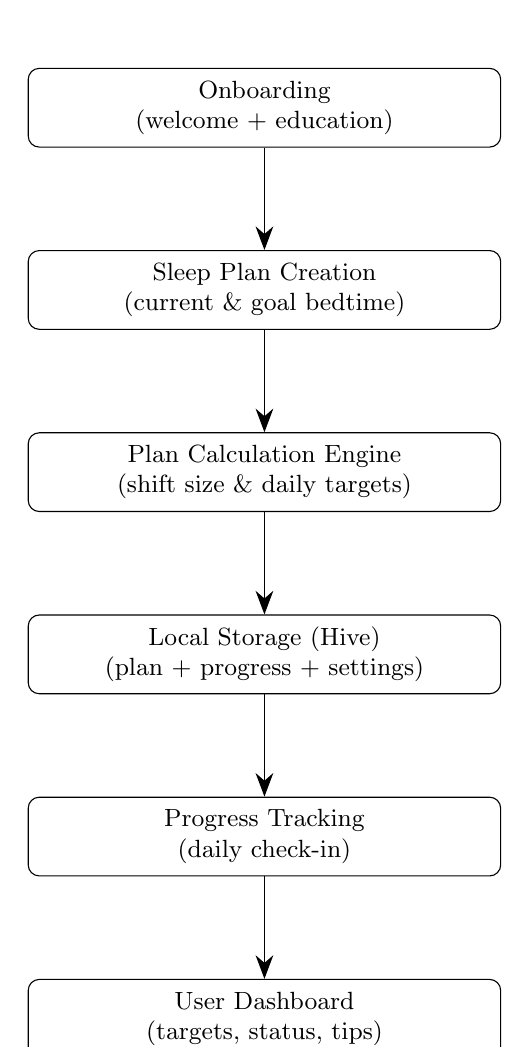
\begin{tikzpicture}[
    node distance=1.3cm,
    box/.style={
        rectangle,
        draw,
        rounded corners,
        minimum width=6cm,
        minimum height=1cm,
        align=center
    },
    >={Stealth[length=3mm]},
    every node/.style={font=\small}
]

\node[box] (onboarding) {Onboarding\\(welcome + education)};
\node[box, below=of onboarding] (plancreate) {Sleep Plan Creation\\(current \& goal bedtime)};
\node[box, below=of plancreate] (planengine) {Plan Calculation Engine\\(shift size \& daily targets)};
\node[box, below=of planengine] (storage) {Local Storage (Hive)\\(plan + progress + settings)};
\node[box, below=of storage] (progress) {Progress Tracking\\(daily check-in)};
\node[box, below=of progress] (dashboard) {User Dashboard\\(targets, status, tips)};

\draw[->] (onboarding) -- (plancreate);
\draw[->] (plancreate) -- (planengine);
\draw[->] (planengine) -- (storage);
\draw[->] (storage) -- (progress);
\draw[->] (progress) -- (dashboard);

\end{tikzpicture}
\caption{High-level workflow of the Sleep Fixer app}
\end{figure}
The system workflow is shown in Figure 1. The main steps are:
\begin{enumerate}
    \item User completes onboarding screens.
    \item User creates a sleep plan by entering current and goal bedtimes.
    \item The app calculates a plan with daily bedtime targets.
    \item The plan is saved locally in a Hive database.
    \item Each day, the user enters their actual bedtime.
    \item The app compares target vs. actual times and assigns a status.
    \item The dashboard shows overall progress and helpful sleep tips.
\end{enumerate}

\subsection{Main Components}

\subsubsection{Presentation Layer (Flutter UI)}
\begin{itemize}
    \item \textbf{OnboardingScreen}: Introduces the app.
    \item \textbf{PlanCreationScreen}: Allows users to enter bedtime information.
    \item \textbf{FullPlanScreen}: Shows the list of bedtime targets.
    \item \textbf{ProgressTrackingDialog}: User inputs actual bedtime.
    \item \textbf{ProfileScreen}: Shows settings and plan summary.
\end{itemize}

\subsubsection{Business Logic Layer}
\begin{itemize}
    \item \textbf{SleepPlanCalculator}: Creates daily bedtime targets.
    \item \textbf{ProgressTrackingService}: Calculates progress status.
    \item \textbf{TimeCalculationUtils}: Helper functions for time differences.
\end{itemize}

\subsubsection{Data Layer}
\begin{itemize}
    \item \textbf{HiveService}: Opens and manages Hive database boxes.
    \item \textbf{SleepPlan Model}: Stores plan information.
    \item \textbf{SleepProgress Model}: Stores daily progress entries.
\end{itemize}

\newpage

% ---------------------------------------------------------------
\section{Core Design Details}

\subsection{Data Storage (Hive Database)}
The app uses Hive, a lightweight NoSQL database stored on the user’s device.  
Two boxes are used:

\begin{itemize}
    \item \textbf{sleep\_progress}: Stores daily progress (date, target time, actual time, status, notes).
    \item \textbf{sleep\_settings}: Stores plan configuration (current bedtime, goal bedtime, shift size, etc.).
\end{itemize}

\subsubsection{Example Progress Entry}
\begin{verbatim}
{
 "date": "2025-12-02",
 "targetTime": "22:00",
 "actualTime": "22:15",
 "status": "within30Min",
 "notes": "Felt good tonight"
}
\end{verbatim}

\subsubsection{Example Sleep Plan}
\begin{verbatim}
{
 "currentBedtime": "23:30",
 "goalBedtime": "22:00",
 "shiftSize": 20,
 "planLength": 9,
 "startDate": "2025-12-01"
}
\end{verbatim}

\subsection{Key Algorithms}

\subsubsection{Shift Size Calculation}
\begin{verbatim}
IF time difference <= 60 minutes → shift = 15 minutes
ELSE IF <= 180 minutes → shift = 20 minutes
ELSE → shift = 30 minutes
\end{verbatim}

\subsubsection{Plan Duration}
\begin{verbatim}
shiftsNeeded = CEILING(totalDifference / shiftSize)
daysPerShift = 1 if difference <= 120 min else 2
totalDays = shiftsNeeded × daysPerShift
\end{verbatim}

\subsubsection{Progress Status Rules}
\begin{verbatim}
0 minutes difference → onTarget
<= 30 minutes → within30Min
<= 60 minutes → within1Hour
> 60 minutes → offTarget
\end{verbatim}

\newpage

% ---------------------------------------------------------------
\section{User Interface Design}

\subsection{Using the App}
\begin{enumerate}
    \item The onboarding screens explain how gradual sleep shifts work.
    \item The user enters their starting and goal bedtime.
    \item The app shows the calculated schedule.
    \item Each day, the user taps the current day and enters their actual bedtime.
    \item The dashboard displays progress and sleep tips.
\end{enumerate}

\subsection{Navigation Layout}
\begin{itemize}
    \item \textbf{Home}: Shows daily targets and progress.
    \item \textbf{Profile}: Shows plan summary and settings.
\end{itemize}

\newpage

% ---------------------------------------------------------------
\section*{Glossary}
\addcontentsline{toc}{section}{Glossary}

\begin{itemize}
    \item SDD - Software Design Document
    \item UI - User Interface
    \item MVP - Minimum Viable Product
    \item API - Application Programming Interface
\end{itemize}

\newpage

% ---------------------------------------------------------------
\section*{References}
\addcontentsline{toc}{section}{References}

\begin{itemize}
    \item Flutter Documentation — \texttt{https://docs.flutter.dev}
    \item Hive Database Documentation — \texttt{https://docs.hivedb.dev}
    \item Dart Language Guides — \texttt{https://dart.dev/guides}
    \item National Sleep Foundation — \texttt{https://www.sleepfoundation.org}
    \item Harvard Medical School Sleep Research — \texttt{https://sleep.med.harvard.edu}
    \item Material Design Guidelines — \texttt{https://material.io/design}
\end{itemize}

\end{document}